\documentclass[a4paper,10pt]{article}
\usepackage[utf8]{inputenc}
%\usepackage[T1]{fontenc}
\usepackage{hyperref}
\usepackage{graphicx}
\graphicspath{{./images}}

\hypersetup{
    colorlinks=true,
    linkcolor=blue,
    filecolor=magenta,      
    urlcolor=cyan,
}

\urlstyle{same}

%opening
\title{Saobraćajne nesreće u Francuskoj od 2005. do 2016. godine}
\author{Jovan Ležaja \\ 
	473/2018 \\
	Matematički fakultet, Beograd \\
	navoj96@gmail.com \\
	\\
	Aleksandar Vračarević \\
	434/2016 \\
	Matematički fakultet, Beograd \\
	vracarevicaleksandar@gmail.com}

\begin{document}

\maketitle

\section{Uvod}
Ovaj rad se fokusira na analizu skupa podataka o saobraćajnim nesrećama u Francuskoj od 2005. do 2006. godine. Pozabavićemo se opisom, 
analizom i pretprocesiranjem datih podataka, a potom ćemo različitim algoritmima pokušati da pronadjemo pravila pridruživanja 
(eng. \textit{Association rules}) koristeći se alatima koje nudi IBM SPSS Modeler.

\section{Opis podataka}

Podaci su preuzeti sa \href{https://www.kaggle.com/ahmedlahlou/accidents-in-france-from-2005-to-2016}{https://www.kaggle.com/ahmedlahlou/accidents-in-france-from-2005-to-2016}
i predstavljaju podatke o saobraćajnim nesrećama u Francuskoj prikupljene u period od 2005. do 2016. godine. Kako bismo uopšte pristupili istraživanju skrivenih pravila u okviru ovog skupa, najpre se moramo upoznati sa istim. Naime, skup se sastoji od 5 tabela u \texttt{.csv} formatu. U nastavku ćemo opisati atribute svake od njih. \\



\begin{itemize}
 \item \texttt{caracteristics.csv}
 \begin{itemize}
  \item \textbf{Num\_Acc} : identifikator nesreće - numerički
  \item \textbf{jour} : dan u mesecu - numerički [1-31]
  \item \textbf{mois} : mesec - numerički [1-12]
  \item \textbf{an} : poslednje dve cifre godine - numerički [5-16]
  \item \textbf{hrmn} : vreme u formatu (ssmm) - numerički [1-2.36k]
  \item \textbf{lum} : osvetljenje u trenutku nesreće brojevi [1-5] kodirani na sledeći način:
			\begin{itemize}
			 \item 1 - dan
			 \item 2 - sumrak/zora
			 \item 3 - noć bez prisutnog javnog osvetljenja
			 \item 4 - noć sa isključenim javnim osvetljenjem
			 \item 5 - noć sa uključenim javnim osvetljenjem
			\end{itemize}
  \item \textbf{dep} : INSEE kod odeljenja praćen nulom %TODO: opisati bolje
  \item \textbf{com} : kod opštine izdat od strane INSEE
  \item \textbf{agg} : \begin{itemize} %TODO: 
                        \item 1 - izvan gradske sredine
                        \item 2 - unutar gradske sredine
                       \end{itemize}
  \item \textbf{int} : tip raskrsnice [1-9] kodirani na sledeći način:
			\begin{itemize}
			 \item 1 - van raskrsnice
			 \item 2 - X raskrsnica
			 \item 3 - T raskrsnica
			 \item 4 - Y raskrsnica
			 \item 5 - raskrsnica sa više od 4 kraka
			 \item 6 - kružni tok
			 \item 7 - place %TODO: sta je ovo
			 \item 8 - pružni prelaz
			 \item 9 - ostalo
			 
			\end{itemize}

  \item \textbf{atm} : atmosferski uslovi [1-9] kodirani na sledeći način:
			\begin{itemize}
			 \item 1 - normalni
			 \item 2 - slaba kiša
			 \item 3 - jaka kiša 
			 \item 4 - sneg/gr\^ad
			 \item 5 - magla/dim
			 \item 6 - jak vetar/oluja
			 \item 7 - zaslepljujuće vreme %TODO: š t a
			 \item 8 - oblačno
			 \item 9 - ostalo
			\end{itemize}
			
  \item \textbf{col} : tip sudara [1-7] kodiran na sledeći način:
			\begin{itemize}
			 \item 1 - čeoni sudar
			 \item 2 - sudar otpozadi
			 \item 3 - sudar sa strane
			 \item 4 - lančani sudar
			 \item 5 - višestruki sudari (više vozila i više sudara)
			 \item 6 - drugi sudari
			 \item 7 - nesreća bez sudara
			\end{itemize}
  
  \item \textbf{adr} : poštanska adresa - niska (popunjava se samo za gradske sredine)
  \item \textbf{gps} : GPS kod - jedan karakter:
			\begin{itemize}
			 \item M - Métropole
			 \item A - Antilles (Martinique or Guadeloupe)
			 \item G = Guyane
			 \item R = Réunion
			 \item Y = Mayotte
			\end{itemize}
			
  \item \textbf{lat} : geografska širina izražena u broju stepeni
  \item \textbf{long} : geografska dužina izražena u broju stepeni



 \end{itemize}

 \item \texttt{holidays.csv}
 \begin{itemize}
  \item \textbf{ds} : datum nesreće u formatu godina-mesec-dan
  \item \textbf{holiday} : naziv praznika
 \end{itemize}
 
 \item \texttt{places.csv}
 \begin{itemize}
  \item \textbf{Num\_Acc} : identifikator nesreće - numerički
  \item \textbf{catr} : kategorija puta [1-9] kodirani na sledeći način:
	\begin{itemize}
	 \item 1 - autoput
	 \item 2 - državni put
	 \item 3 - departmentalni putevi
	 \item 4 - komunalni putevi
	 \item 5 - mreža puteva zabranjena za javnost
	 \item 6 - javni parking
	 \item 9 - ostalo
	\end{itemize}
  \item \textbf{voie} : broj puta - numerički
  \item \textbf{V1} : numerički indeks broja puta (na primer: 2 bis, 3 ter itd.)
  \item \textbf{V2} : alfanumerički indeks puta
  \item \textbf{circ} : tip saobraćanja [1-4] kodiran na sledeći način:
	\begin{itemize}
	 \item 1 - jednosmerna ulica
	 \item 2 - dvosmerna ulica
	 \item 3 - razdvojen kolovoz
	 \item 4 - 
	\end{itemize}
  \item \textbf{nbv} : ukupan broj traka na putu - numerički
  \item \textbf{vosp} : indikator postojanja rezervisane trake [1-3], 
			nezavisno od toga da li se nesreća dogodila u toj traci, kodiran na sledeći način:
	\begin{itemize}
	 \item 1 - bickilistička traka
	 \item 2 - parking za bicikle
	 \item 3 - rezervisan kanal
	\end{itemize}
  \item \textbf{prof} : kategorije puta [1-4] zavisno od nagiba puta, kodirane na sledeći:
	\begin{itemize}
	 \item 1 - ``dish''
	 \item 2 - nizbrdica
	 \item 3 - vrh brda
	 \item 4 - dno brda
	\end{itemize}
  \item \textbf{pr} : PR broj kuće - numerička vrednost
  \item \textbf{pr1} : udaljenost od najbližeg PR broja izražena u metrima - numerička vrednost
  \item \textbf{plan} : izgled puta na mapi [1-4], kodirano na sledeći način:
	\begin{itemize}
	 \item 1 - prav put
	 \item 2 - zakrivljen ulevo
	 \item 3 - zakrivljen udesno
	 \item 4 - ``S'' oblika
	\end{itemize}
  \item \textbf{lartpc} : širina ostrva na ulici, ako postoji - niska
  \item \textbf{larrout} : širina puta namenjena za saobraćaj - niska
  \item \textbf{surf} : stanje terena [1-9], kodiran na sledeći način:
	\begin{itemize}
	 \item 1 - normalan
	 \item 2 - vlažan
	 \item 3 - teren
	 \item 4 - potopljen
	 \item 5 - sneg na terenu
	 \item 6 - blatnjav
	 \item 7 - poledica na terenu
	 \item 8 - masan/zauljen teren
	 \item 9 - ostalo
	\end{itemize}
  \item \textbf{infra} : infrastruktura puteva [1-7], kodirana na sledeći način:
	\begin{itemize}
	 \item 1 - podzemni tunel
	 \item 2 - most/nadvožnjak
	 \item 3 - uključenje
	 \item 4 - pruga
	 \item 5 - ``carrefour arranged''
	 \item 6 - pešačka zona
	 \item 7 - ostalo
	\end{itemize}
  \item \textbf{situ} : pozicija nesreće [1-5], kodirana na sledeći način:
	\begin{itemize}
	 \item 1 - na putu
	 \item 2 - u zaustavnoj traci
	 \item 3 - na ivičnjaku
	 \item 4 - na trotoaru
	 \item 5 - na biciklističkoj stazi
	\end{itemize}
  \item \textbf{env1} : locirano blizu škole - numerička vrednost
 \end{itemize}

 \item \texttt{users.csv}
 \begin{itemize}
  \item \textbf{Acc\_number} : identifikator nesreće - numerički
  \item \textbf{Num\_Veh} : identifikator vozila - alfanumerički
  \item \textbf{place} : pozicija osobe u vozilu u vreme nesreće, kodirano u skladu sa sledećom slikom:
  
\begin{minipage}{0.7\textwidth}
 \centering
 \makebox[\textwidth][c]{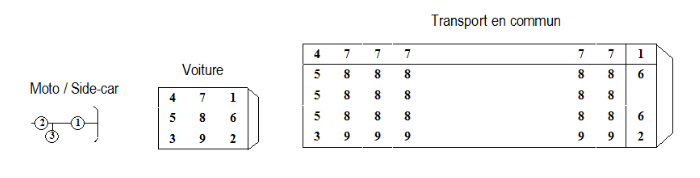
\includegraphics[width=\textwidth]{./images/ip_sem_img_4.png}}
\end{minipage}
  
  \item \textbf{catu} : uloga osobe u saobraćaju u trenutku nesreće [1-4], kodirano na sledeći način:
	\begin{itemize}
	 \item 1 - vozač
	 \item 2 - putnik
	 \item 3 - pešak
	 \item 4 - pešak na rolerima ili skuteru
	\end{itemize}
  \item \textbf{grav} : ozbiljnost povrede [1-4], kodirana na sledeći način:
	\begin{itemize}
	 \item 1 - neozledjen
	 \item 2 - ubijen
	 \item 3 - hospitalizovan
	 \item 4 - blaga ozleda
	\end{itemize}
  \item \textbf{sex} : pol osobe:
	\begin{itemize}
	 \item 1 - muško
	 \item 2 - žensko
	\end{itemize}
  \item \textbf{Year\_on} : godina rodjenja - numerički
  \item \textbf{trip} : razlog putovanja [1-9], kodiran na sledeći način:
	\begin{itemize}
	 \item 1 - kuća-posao
	 \item 2 - posao-kuća
	 \item 3 - kupovina
	 \item 4 - poslovni put
	 \item 5 - razonoda
	 \item 9 - ostalo
	\end{itemize}
  \item \textbf{secu} : niska koja se sastoji od 2 broja. 
			Prvi označava postojanje sigurnosne opreme [1-9], kodirano na sledeći način:
	\begin{itemize}
	 \item 1 - pojas za vezivanje
	 \item 2 - kaciga
	 \item 3 - sedeljka za decu
	 \item 4 - reflektujuća oprema
	 \item 9 - ostalo
	\end{itemize}
	
	Drugi označava korišćenje sigurnosne opreme [1-3], kodirano na sledeći način:
	\begin{itemize}
	 \item 1 - oprema je korišćena
	 \item 2 - oprema nije korišćena
	 \item 3 - neodredjeno
	\end{itemize}

  \item \textbf{locp} : pozicija pešaka [1-8], kodirano na sledeći način:
	\begin{itemize}
	 \item 1 - više od 50 metara od pešačkog prelaza
	 \item 2 - manje od 50 metara od pešačkog prelaza
	 \item 3 - na pešačkom prelazu sa semaforom
	 \item 4 - na pešačkom prelazu bez semafora
	 \item 5 - na trotoaru
	 \item 6 - na ivičnjaku
	 \item 7 - pod zaklonom
	 \item 8 - u prolazu
	\end{itemize}

  \item \textbf{actp} : akcija pešaka [0-9], kodirano na sledeći način:
	\begin{itemize}
	 \item 0 - neodredjeno
	 \item 1 - kreće se u istom smeru kao i vozilo sa kojim se dogodio sudar
	 \item 2 - kreće se u suprotnom smeru kao i vozilo sa kojim se dogodio sudar
	 \item 3 - prelazak ulice
	 \item 4 - zaklonjen
	 \item 5 - u trku
	 \item 6 - sa životinjom
	 \item 9 - ostalo
	\end{itemize}

  \item \textbf{etatp} : kategorička vrednost koja odredjuje da li je pešak bio u društvu drugih ljudi ili ne, kodirano na sledeći način:
	\begin{itemize}
	 \item 1 - sam
	 \item 2 - sa saputnikom
	 \item 3 - u grupi ljudi
	\end{itemize}

 \end{itemize}
 
 \item \texttt{vehicles.csv}
 \begin{itemize}
  \item \textbf{Num\_Acc} : identifikator nesreće - numerički
  \item \textbf{Num\_veh} : identifikator vozila - alfanumerički kod
  \item \textbf{GP} : %TODO: š t a
  \item \textbf{CATV} : kategorija vozila [01 - 13]
		      \begin{itemize}
		       \item 01 - bicikl
		       \item 02 - moped < 50 kubika
		       \item 03 - kvadricikl sa motorom
		       \item 04 - suvišno od 2006. (registrovani skuter)
		       \item 05 - suvišno od 2006. (motocikl)
		       \item 06 - suvišno od 2006. (putnička prikolica za motocikl)
		       \item 07 - VL %TODO: tebra
		       \item 08 - neupotrebljena kategorija (VL i karavan)
		       \item 09 - neupotrebljena kategorija (VL i prikolica)
		       \item 10 - VU %TODO: nmg
		       \item 11 - najviše korišćeno posle 2006. godine (VU(10) + karavan)
		       \item 12 - najviše korišćeno posle 2006. godine (VU(10) + prikolica)
		       \item 13 - PL samo 3.5T
		       \item 14 - 
		      \end{itemize}

 \end{itemize}
 
\end{itemize}

\section{Analiza i pretprocesiranje podataka}
Prilikom učitavanja tabele \textit{characteristics} smo uočili da je usled loše formatirane datoteke došlo do pogrešne reprezentacije podataka, što smo razrešili jednostavnom \textit{Python} skriptom.
Analizirajući tabelu \texttt{characteristics} uočili smo da atributi \textit{gps}, \textit{lat} i \textit{long} imaju značajan broj 
nedostajućih vrednosti (preko 50\%), a s obzirom da zamena nekom konkretnom vrednošću nema smisla zato što nemamo dovoljno validnih vrednosti u koloni da njihova zamena bude smislena,
odlučili smo da ih uklonimo, jer smatramo da nam nisu bitni za dalju analizu. Kada je reč o atributima \textit{atm} i \textit{col}, 
zbog izuzetno malog broja nedostajućih vrednosti (atributi su bili kompletni blizu 100\%), u čvoru \textit{Type} smo ih odbacili, 
jer ne gubimo ništa odbacivanjem tako malog broja podataka. U tabeli se isto tako nalaze i atributi vezani za lokaciju nesreća (ulica, opština, itd.),
ali dodatnim posmatranjem smo primetili da je format zapisa tih podataka dosta nekonzistentan, tako da je njihova korisnost dovedena u pitanje,
pošto bez iscrpnog analiziranja teksta ne bismo mogli da izvučemo korisne informacije, što je dovelo do odluke da preko čvora \textit{Type} 
tim atributima postavimo ulogu (``Role'') na vrednost \texttt{None}.

\begin{figure}[h!]
 \centering
 \makebox[\textwidth][c]{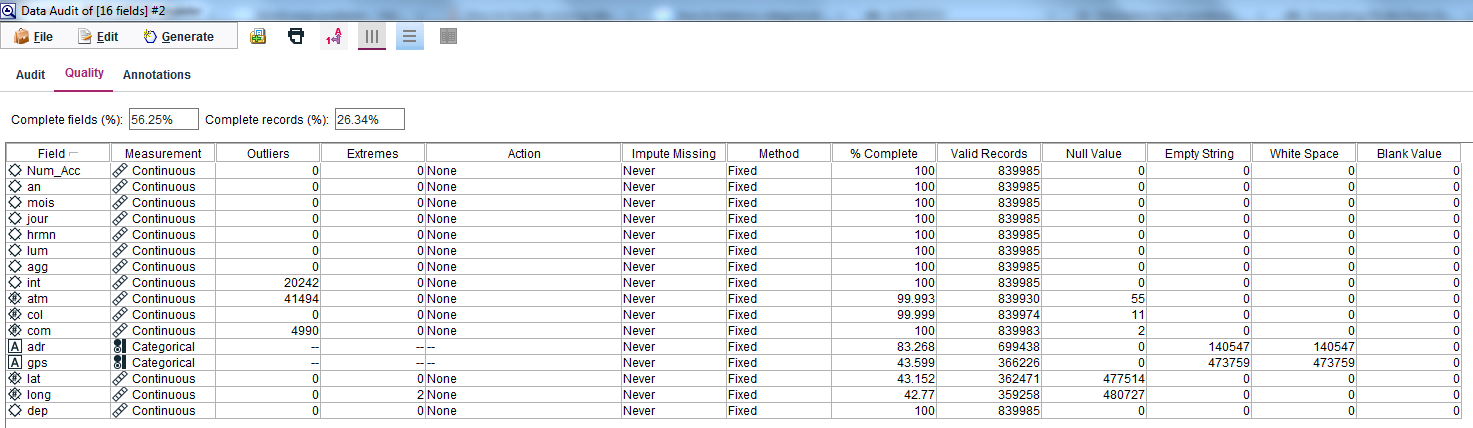
\includegraphics[width=1.4\textwidth,height=0.25\textheight]{./images/ip_sem_img_1.png}}
 \caption{Sadržaj \textit{Data Audit} čvora za tabelu \texttt{characteristics}}
\end{figure}

\begin{figure}[h!]
 \centering
 \makebox[\textwidth][c]{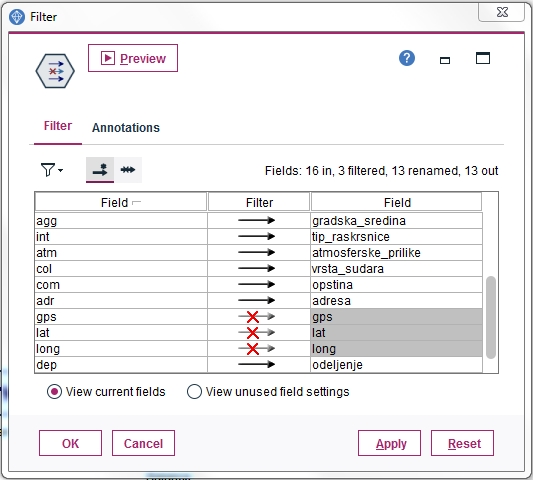
\includegraphics[width=0.55\textwidth]{./images/ip_sem_img_2.png}}
 \caption{Sadržaj \textit{Filter} čvora za tabelu \texttt{characteristics}}
\end{figure}

\begin{figure}[h!]
 \centering
 \makebox[\textwidth][c]{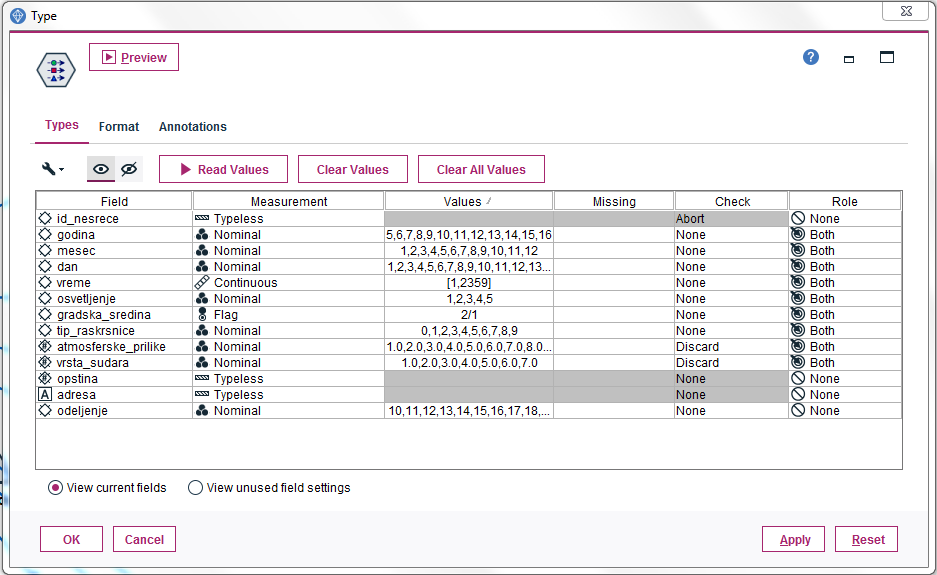
\includegraphics[width=1.3\textwidth,height=0.5\textheight]{./images/ip_sem_img_3.png}}
 \caption{Sadržaj \textit{Type} čvora za tabelu \texttt{characteristics}}
\end{figure}

Analizom skupa podataka \texttt{users} uočili smo da atributi \textit{locp}, \textit{actp} i \textit{etatp}, koji predstavljaju informacije vezane
za pešaka, imaju značajan broj neodredjenih vrednosti (preko 50\%), tako da smo te kolone izbacili iz skupa podataka \textit{users}. Kada je u pitanju
atribut \textit{secu}, čije su vrednosti predstavljene kao dva broja, uočili smo nekonzistentnost odredjenih polja sa zadatim opisom reprezentacije tog atributa,
tako da smo te nekonzistentne vrednosti preimenovali u \texttt{NA} (neodredjenu vrednost). Za svaki atribut koji je imao 0 kao vrednost, a nije bilo definisano
šta ta vrednost predstavlja, 0 je zamenjena sa \texttt{NA}. Za atribut \textit{place} smo sve vrednosti ostavili kakve jesu, pošto je šema 
koja predstavlja kodiranje bila nedovoljno jasna.

Skup podataka \texttt{vehicles} smo analizirali i zaključili da sve slogove koji sadrže nedostajuće i neodredjene 
vrednosti možemo da odbacimo. Nismo naišli ni na kakve nepravilnosti koje iziskuju podrobnije procesiranje.

Nakon što smo uvideli da kolone \texttt{v1} i \texttt{v2} skupa \texttt{places} sadrže ogroman broj nedostajućih
vrednosti, odbacili smo ih. Pošto se u kolonama \texttt{pr} i \texttt{pr1} javlja preko 50\% nedostajućih vrednosti, a smatramo da ne postoji
smislen način da te vrednosti popunimo, odbacili smo i ove kolone. Kolona \texttt{env1} predstavlja predstavlja meru blizine
školi, ali je zbog nejasnog kodiranja i ova kolona odbačena. Iako kolone \texttt{voie}, \texttt{vosp}, \texttt{lartpc}, \texttt{infra}
i \texttt{nbv} nemaju puno nedostajućih vrednosti, gotovo svi slogovi uzimaju mali skup vrednosti za pomenute atribute pa smo 
se odlučili da ni ove atribute ne koristimo u daljoj analizi. Za kolone \texttt{situ}, \texttt{prof}, \texttt{surf} i \texttt{plan}
ćemo odbaciti slogove sa vrednošću nula za ove atribute. U koloni \texttt{larrout} se javljaju negativne vrednosti za širinu
puta, pa ćemo i njih ukloniti.

Skup podataka \texttt{holidays} smo odlučili da ne koristimo za dalju analizu, jer ne sadrži preterano korisne informacije.

\section{Pravila pridruživanja}
Nakon što smo obradili skupove podataka, hteli smo da na svaki od relevantnih skupova primenimo algoritme \textit{Apriori} i \textit{Carma},
u nadi da ćemo uočiti neka zanimljiva pravila. Nakon primene pomenutih algoritama, cilj nam je bio da primenimo iste algoritme nad objedinjenim podacima.

\subsection{Primena \textit{Apriori} i \textit{Carma} algoritama nad skupom \texttt{characteristics}}
Iskoristili smo niz čvorova \textit{Reclassify} kako bismo lakše tumačili kategoričke vrednosti. Iz tog skupa smo filtrirali one slogove čija je 
vrednost atributa \textit{tip\_raskrsnice} \texttt{NA}. Potom smo primenili \textit{Apriori} sa podrazumevanim podešavanjima 
(minimalna podrška uzročnika je 10\%, a minimalna pouzdanost pravila je 80\%) i rezultati izvršavanja
tog algoritma se mogu videti na slici. Posledice pravila se odnose na atmosferske prilike, tip raskrsnice i indikator da li se nesreća desila u gradu ili ne.
Algoritam je uspeo da nadje 30 pravila, koja sve u svemu nisu zanimljiva. Naime, lift mera se kreće u opsegu od 0.998 do 1.314, što nam govori da su
uzročnici u blagoj korelaciji sa posledicama. Kako bismo pripremili skup podataka za algoritam \textit{Carma}, koristili smo čvor \textit{SetToFlag}. 
\textit{Carma} algoritam smo primenili sa istim parametrima kao i \textit{Apriori}. Dobili smo 22 pravila, koja su gotovo identična onima koje smo
dobili korišćenjem \textit{Apriori} algoritma. \\
% TODO: slika Apriori(5) i Carma(6)
 
 \begin{figure}[!h]
 \centering
 \makebox[\textwidth][c]{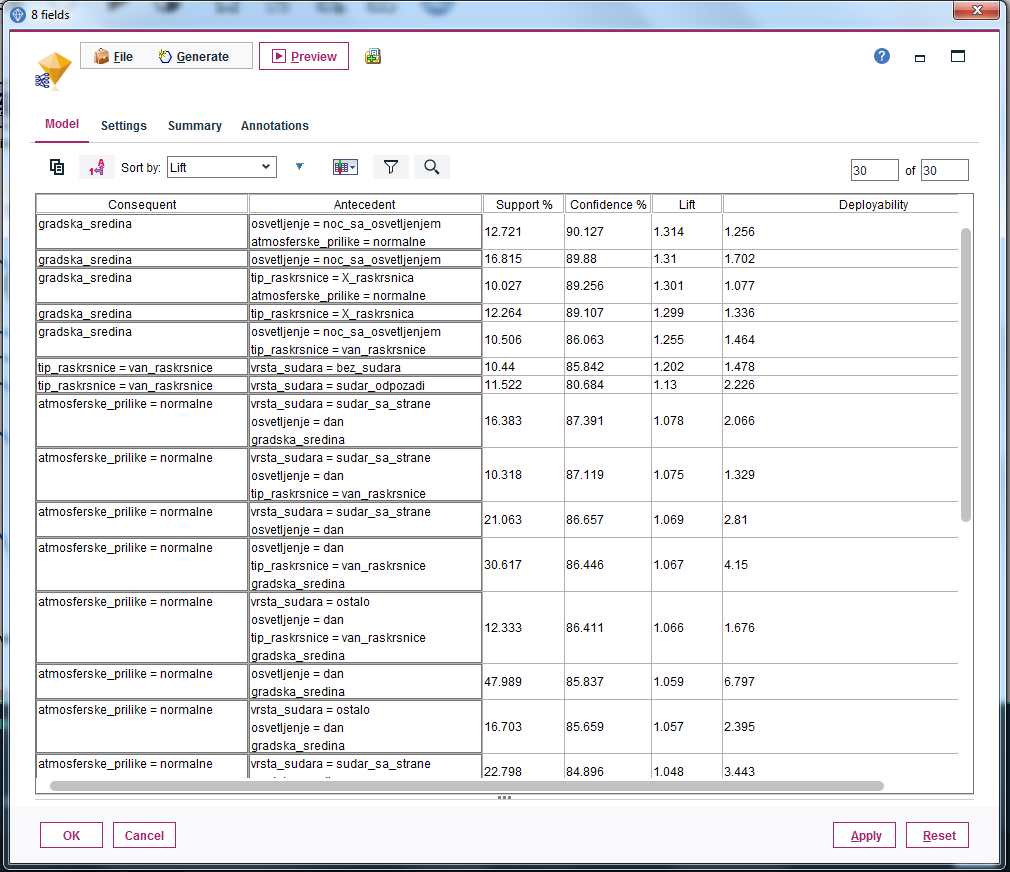
\includegraphics[width=1\textwidth,height=0.3\textheight]{./images/5_rezultati_apriori.PNG}}
 \caption{Apriori}
\end{figure}

\begin{figure}[!h]
 \centering
 \makebox[\textwidth][c]{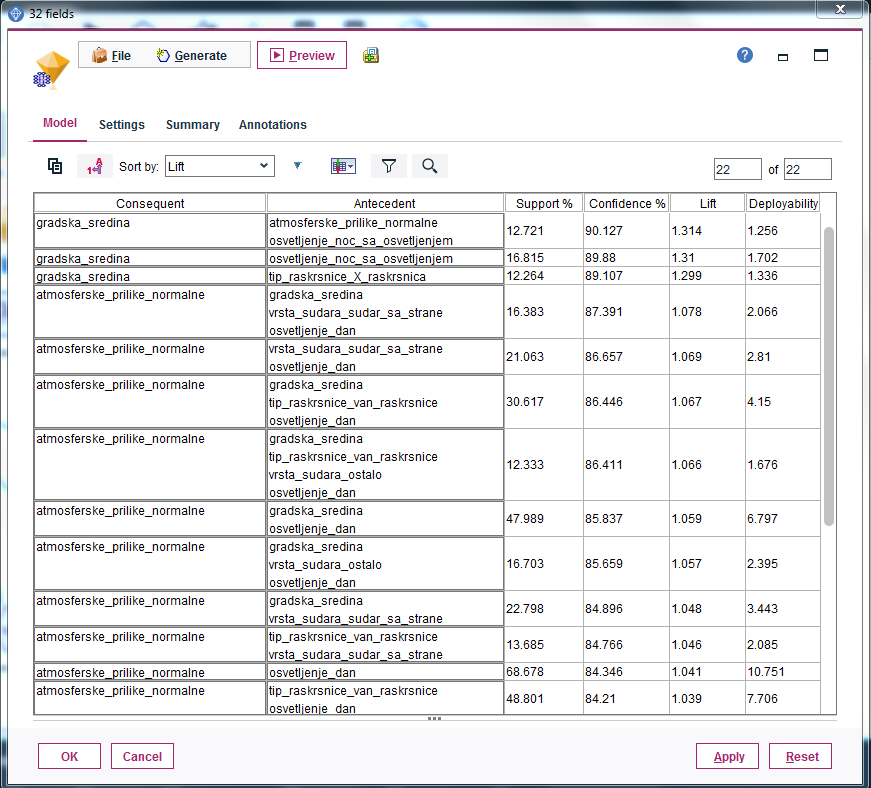
\includegraphics[width=1\textwidth,height=0.3\textheight]{./images/6_rezultati_carma.PNG}}
 \caption{Carma}
\end{figure}
 
Kao što se iz rezultata \textit{Data Audit} čvora može primetiti, odredjene vrednosti nekh atributa dominiraju nad ostalim vrednostima, te stoga ne
čudi što otkrivena pravila sadrže te vrednosti. 
%TODO: slika 7+

\begin{figure}[!h]
 \centering
 \label{fig:data_audit}
 \makebox[\textwidth][c]{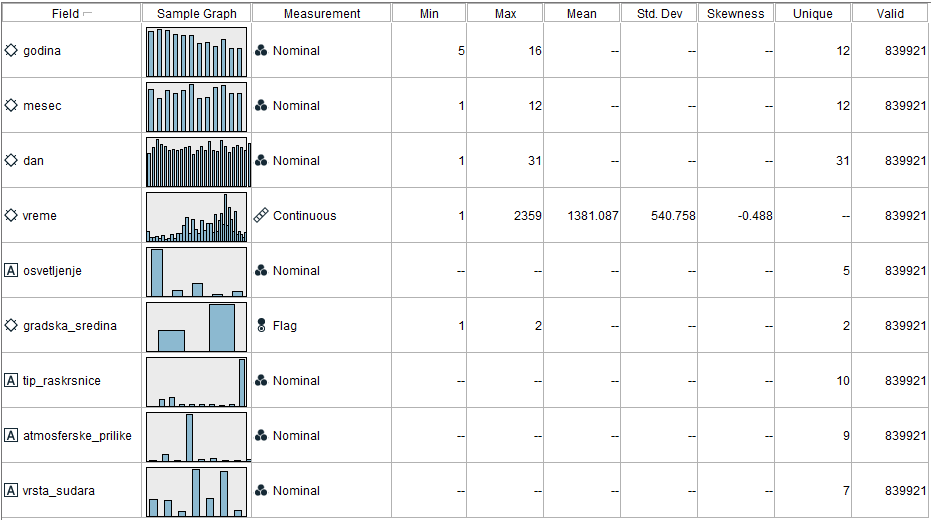
\includegraphics[width=1\textwidth,height=0.3\textheight]{./images/stream1_data_audit_hist.PNG}}
 \caption{Možemo videti da se u kolonama \textit{osvetljenje}, \textit{tip\_raskrsnice} i \textit{atmosferske\_prilike} u 
 najvećem broju slučajeva javlja samo jedna vrednost, te ćemo te vrednosti pokušati da izbalansiramo. Još jedna kolona na koju ćemo 
 primeniti balansiranje je \textit{vrsta\_sudara}.}
\end{figure}

U želji da izbor pravila bude pravedniji, odlučili smo da izbalansiramo skup podataka, tako što 
ćemo korišćenjem čvorova \textit{Balance} na pojedinačne kolone ublažiti efekat dominantnih vrednosti (pomenute čvorove
smo generisali uz pomoć distribucija odgovarajućih kolona). Nakon toga smo redom primenjivali \textit{Apriori}
algoritam za svaku izmenjenu kolonu. Potom smo eksperimentisali sa primenom \textit{Apriori} alogritma na ulančane \textit{Balance} čvorove. 
Neki od rezultata su predstavljeni na narednim slikama.

\begin{figure}[!h]
 \centering
 \makebox[\textwidth][c]{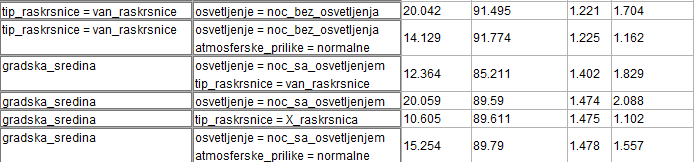
\includegraphics[width=1.3\textwidth,height=0.2\textheight]{./images/stream1_apriori_bal_osvetljenje.PNG}}
 \caption{Rezultat primene apriori algoritma na balansiranu kolonu \textit{osvetljenje}. Izdvojena pravila jesu logična, ali nam 
 ne otkrivaju puno interesantnih zaključaka.}
\end{figure}

\begin{figure}[h!]
 \centering
 \makebox[\textwidth][c]{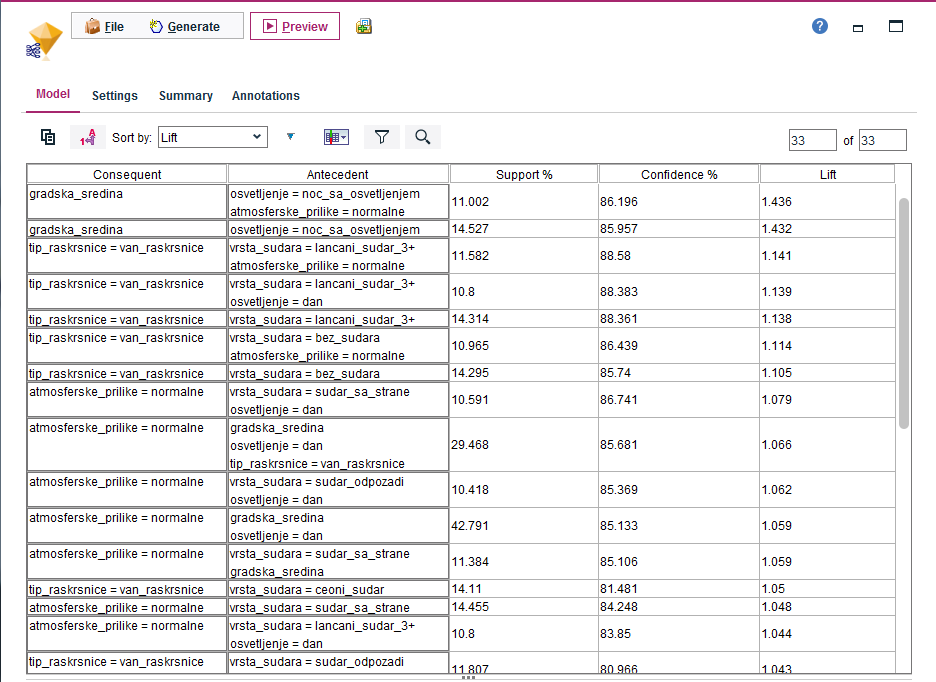
\includegraphics[width=1.3\textwidth,height=0.4\textheight]{./images/stream1_apriori_red_sudar.PNG}}
 \caption{Rezultat primene apriori algoritma na balansiranu kolonu \textit{vrsta\_sudara}. U ovom slučaju je pronadjeno 33 pravila
  od kojih su ona sa najvećom lift merom logična ali i dalje nam ne daju upotrebljiviji uvid u zavisnosti medju atributima. }
\end{figure}

\clearpage
Zaključujemo da balansiranje pojedinačnih kolona ne dovodi do željenih rezultata te smo probali sa ulančanim balansiranjem.

\begin{figure}[!h]
 \centering
 \makebox[\textwidth][c]{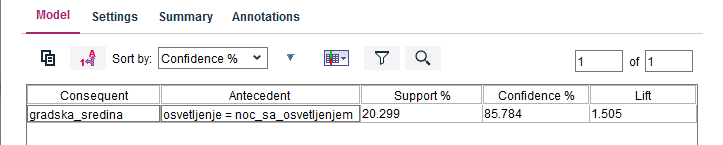
\includegraphics[width=1\textwidth,height=0.1\textheight]{./images/stream1_apriori_bal_osvetljenje_SEQ.PNG}}
 \caption{Rezultat primene apriori algoritma na redom izbalansirane sve kolone skupa. Izdvojeno pravilo prema lift meri jeste
 zanimljivo ali je opet očekivano da u gradskoj sredini postoji osvetljenje koje je uključeno. }
\end{figure}

%stream1_apriori_reduce_atm_SEQ.PNG
\begin{figure}[!h]
 \centering
 \makebox[\textwidth][c]{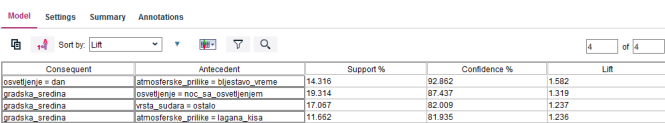
\includegraphics[width=1\textwidth,height=0.1\textheight]{./images/stream1_apriori_reduce_atm_SEQ.PNG}}
 \caption{Rezultat primene apriori algoritma na balansirane kolone \textit{tip\_raskrsnice}, \textit{vrsta\_sudara} 
 i \textit{atmosferske\_prilike}. }
\end{figure}


Kako pokušaj sa balansiranjem nije prošao slavno, odlučili smo se da potpuno eliminišemo slogove koji imaju najzastupljeniju vrednost odredjenog atributa,
i da na njega primenimo iste algoritme. Na ovaj način smo otkrili više pravila nego u prethodnim pokušajima, sa lift merama 
u opsegu od 0.673 do 1.421, ali sa malom pouzdanošću i podrškom. Rezultati se mogu videti na slici.

\begin{figure}[!h]
 \centering
 \makebox[\textwidth][c]{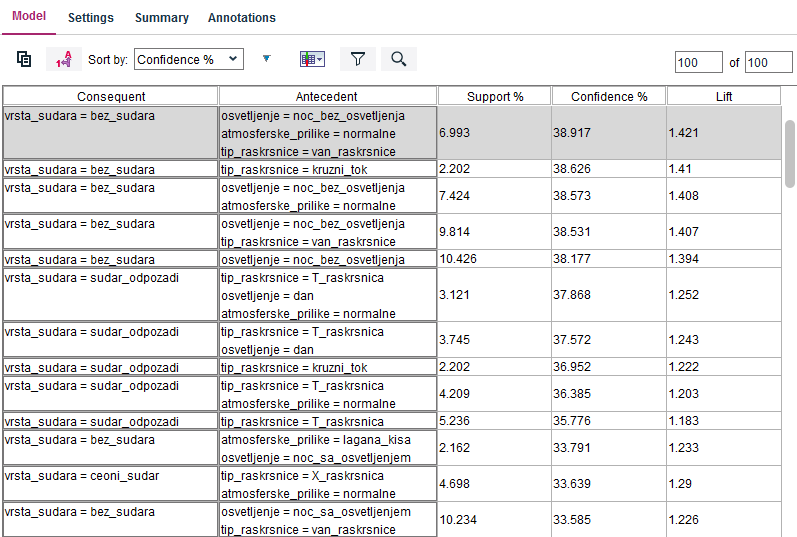
\includegraphics[width=1.1\textwidth,height=0.3\textheight]{./images/stream1_apriori_vrsta_sudara.PNG}}
 \caption{Nakon izbacivanja slogova koji bi `prigušili` ostatak skupa, dobijeni su ovakvi rezultati. I dalje smatramo da ne 
 postoje izuzetno zanimljiva pravila. }
\end{figure}

\clearpage

\begin{figure}[h!]
 \centering
 \makebox[\textwidth][c]{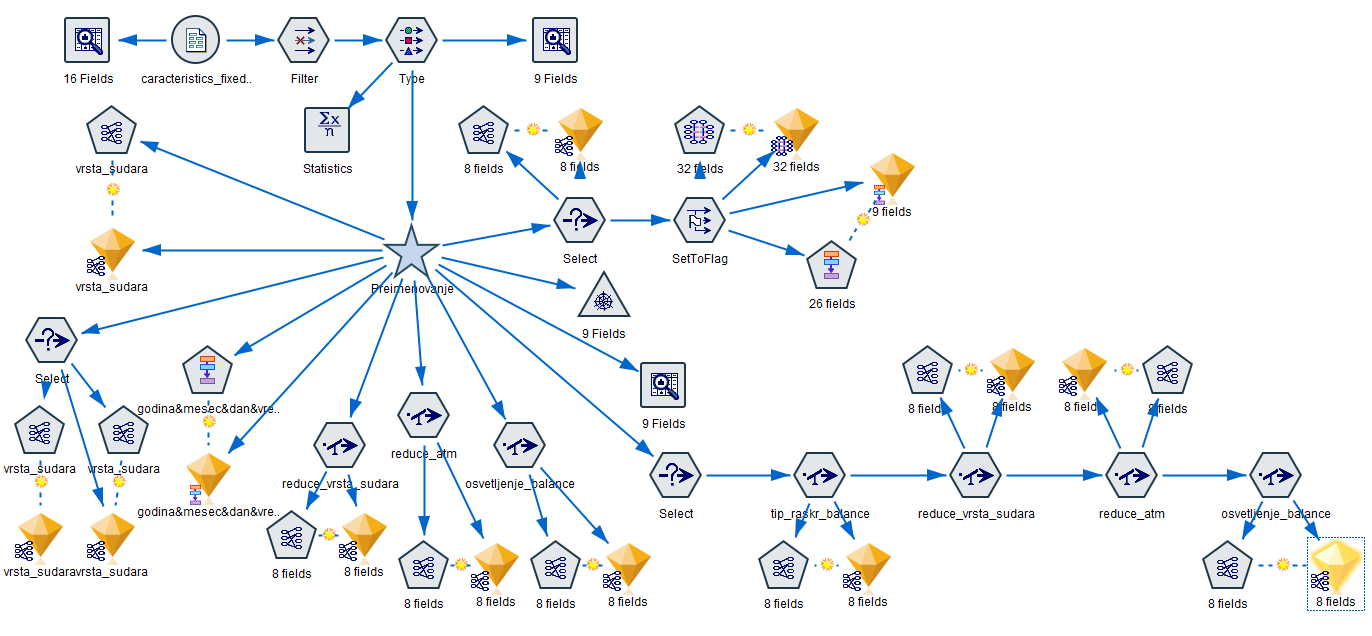
\includegraphics[width=1.3\textwidth,height=0.4\textheight]{./images/stream1_model.PNG}}
 \caption{Prikaz celokupnog streama obrade skupa \textit{caracteristics.csv} }
\end{figure}

%TODO: 	broj putnika: nesto slogirano, brisemo
% 	

\subsection{Primena \textit{Apriori} i \textit{Carma} algoritama nad skupom \texttt{places}}

\subsection{Primena \textit{Apriori} i \textit{Carma} algoritama nad objedinjenim podacima}

Uz pomoć čvora \textit{Merge} smo spojili skupove \textit{users}, \textit{vehicles} i \textit{caracteristics} izbacujući 
redove sa nedostajućim vrednostima usput. Nakon toga smo izbacili kolone ... Izvršili smo dodatno uklanjanje besmislenih slogova
i tako pripremljene podatke propustili kroz \textit{Apriori} i \textit{Carma} čvorove. U prvoj iteraciji smo koristili
podrazumevane parametre za oba čvora. Rezultati su u nastavku.

\begin{figure}[h!]
 \centering
 \makebox[\textwidth][c]{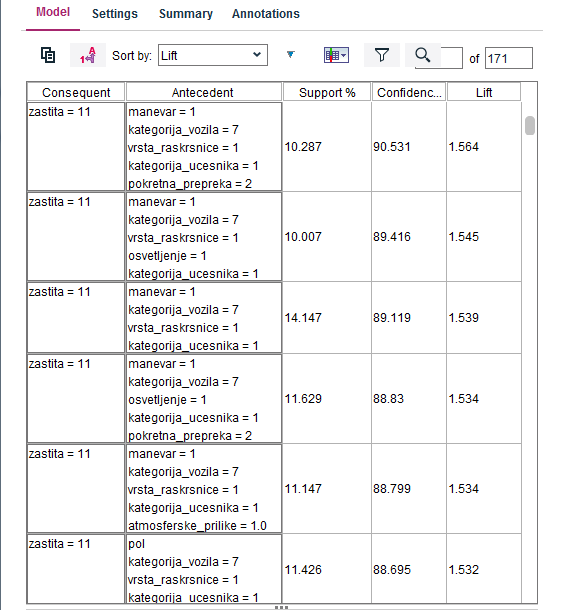
\includegraphics[width=1\textwidth,height=0.3\textheight]{./images/default_apriori.PNG}}
 \caption{Rezultati apriori algoritma sa podrazumevanim parametrima nad objedinjenim skupom.}
\end{figure}

\begin{figure}[h!]
 \centering
 \makebox[\textwidth][c]{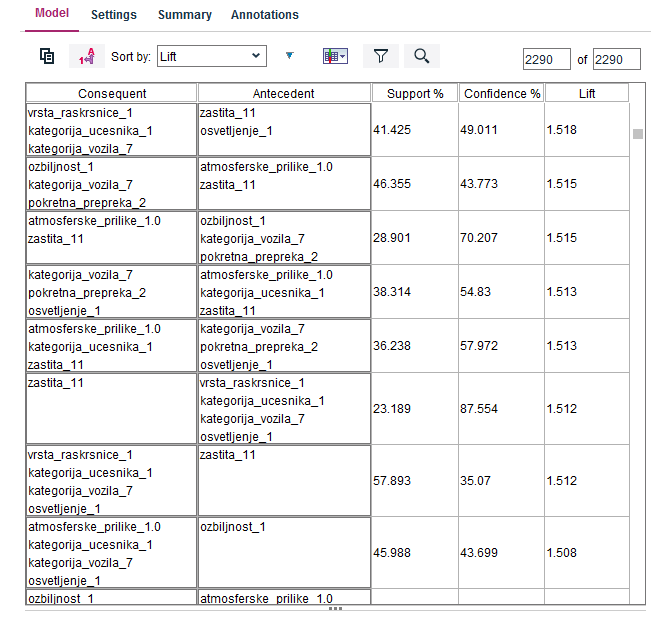
\includegraphics[width=1\textwidth,height=0.3\textheight]{./images/default_carma.PNG}}
 \caption{Rezultati carma algoritma sa podrazumevanim parametrima nad objedinjenim skupom.}
\end{figure}

\clearpage

Primećujemo da su prisutna pravila sa solidnom lift merom od oko 1.5 i velikom podrškom za oba algoritma. Odmah se Primećuje
i ogromna razlika u količini pronadjenih pravila. Većina pravila pronadjenih aprior algoritmom kao posledicu imaju nošenje
zaštitnog pojasa u trenutku nesreće. Kod carma algoritma pravila su malo raznolikija ali i dalje se u pravilima javljaju 
većinski dominantne vrednosti odgovarajućih kolona. U nastavku ćemo pokušati da ispitamo vezu izmedju nekih atributa za koje
mislimo da mogu proizvesti interesantna pravila. \\

Najpre smo hteli da ispitamo postoje li veze izmedju atmosferskih prilika, vrste sudara, kategorija učesnika, ozbiljnosti povreda
i korišćene zaštitne opreme. Kroz više iteracija smo se zaustavili na minimalnoj podršci od 5.0\% i minimalnoj pouzdanosti od 60.0\%.
Pravila dobijena apriorijem kojima je lift mera najveća uglavnom za posledicu imaju nošenje zaštitnog pojasa, pa nam ovo nije 
preterano zanimljivo. 

\begin{figure}[h!]
 \centering
 \makebox[\textwidth][c]{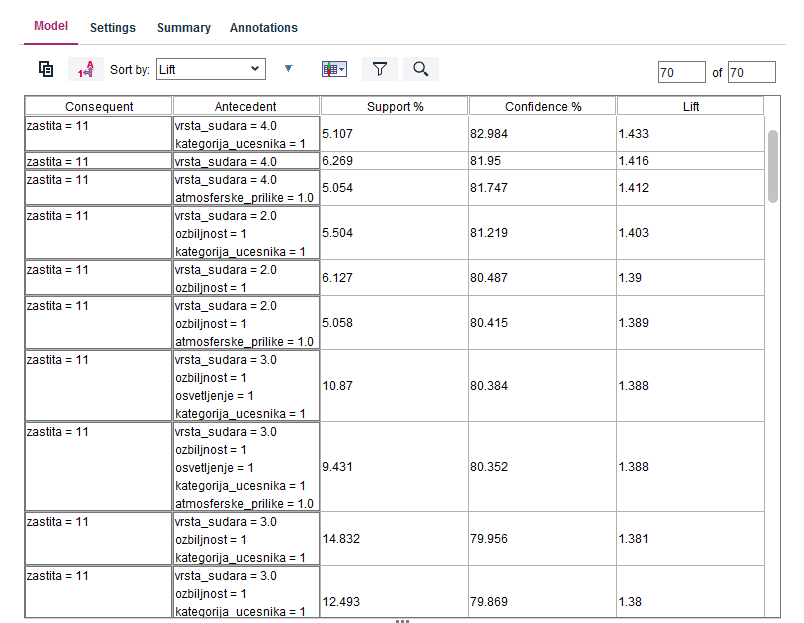
\includegraphics[width=1.3\textwidth,height=0.4\textheight]{./images/jovanov_izbor_apriori.PNG}}
 \caption{Rezultati apriori algoritma primenjenog na atmosferske prilike, vrstu sudara, kategoriju učesnika, ozbiljnost povreda
i korišćenu zaštitnu opremu. }
\end{figure}

Carma algoritam je dao malo zanimljivije rezultate. Naime, pronadjena su tri pravila koja lift merom odstupaju od jedinice. Pravilo
\textit{žensko + korišćen je zaštitni pojas} ima lift meru od 1.128 što nam govori da postoji blaga pozitivna korelacija
izmedju ženskog pola i vezivanja zaštitnog pojasa. S druge strane, na osnovu lift mere manje od 1, dolazimo do zaključka
da ukoliko je došlo do blage ozlede, možemo spekulisati da se ne radi o vozaču. Slično tome, ukoliko je učesnik nezgode 
žensko, manja je šansa da je vozač nego neka druga kategorija učesnika. Za ovaj čvor smo koristili minimalnu podršku od 20.0\% i
minimalnu pouzdanost od 60.0\%. \\

\begin{figure}[h!]
 \centering
 \makebox[\textwidth][c]{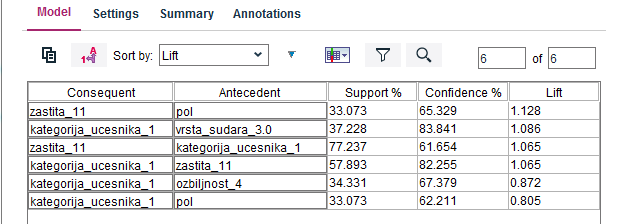
\includegraphics[width=1\textwidth,height=0.15\textheight]{./images/jovanov_izbor_carma.PNG}}
 \caption{Rezultati carma algoritma primenjenog na atmosferske prilike, vrstu sudara, kategoriju učesnika, ozbiljnost povreda
i korišćenu zaštitnu opremu. }
\end{figure} 

Sledeći pokušaj se odnosio na uticaj zaštitne opreme i vrste sudara na ozbiljnost povreda. Carma čvor je ostavljen sa 
podrazumevanim vrednostima (po 20.0\% za oba parametra). Čvoru apriori smo iterativno smanjivali parametre, ali ni za minimalnu
podršku od 5.0\% i minimalnu pouzdanost od 5.0\% nije uspeo da pronadje nijedno pravilo.

\begin{figure}[h!]
 \centering
 \makebox[\textwidth][c]{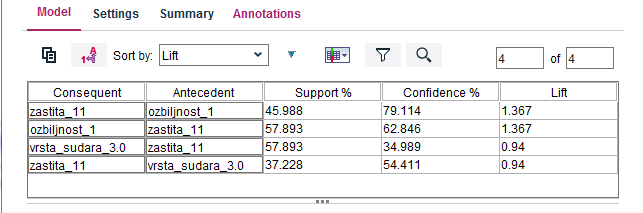
\includegraphics[width=1\textwidth,height=0.15\textheight]{./images/izbor2_carma.PNG}}
 \caption{Rezultati carma algoritma primenjenog na vrstu sudara, zaštitu i ozbiljnost povrede. Jedini zaključak koji
 možemo izvesti je da korišćenje zaštitnog pojasa pozitivno korelira sa odsustvom ozlede. Podrška i lift mera ostala dva pravila
 nam govori da ta pravila nisu dovoljno interesantna. }
\end{figure}

Nakon toga smo se pitali da li kategorija učesnika ima veze sa korišćenom zaštitnom opremom. 

\begin{figure}[h!]
 \centering
 \makebox[\textwidth][c]{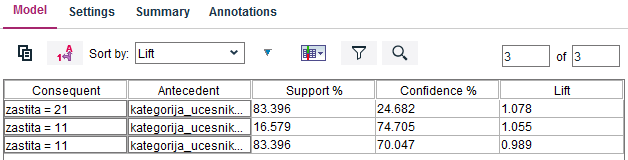
\includegraphics[width=1\textwidth,height=0.15\textheight]{./images/izbor3_apriori.PNG}}
 \caption{Rezultati apriori algoritma primenjenog na kategoriju učesnika i korišćenu zaštitnu opremu. Iz sličnog razloga kao i za 
 apriori odbacujemo ova pravila kao nekorisna. }
\end{figure}

\begin{figure}[h!]
 \centering
 \makebox[\textwidth][c]{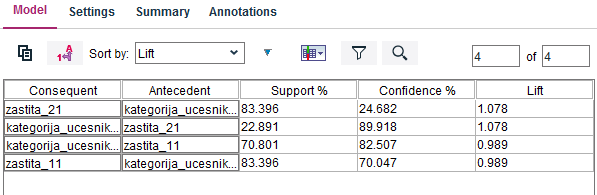
\includegraphics[width=1\textwidth,height=0.15\textheight]{./images/izbor3_carma.PNG}}
 \caption{Rezultati carma algoritma primenjenog na kategoriju učesnika i korišćenu zaštitnu opremu. Lift mera je veoma bliska 
 jedinici te ne smatramo pravila interesantnim. }
\end{figure}

Pitali smo se da li godine učesnika imaju veze sa korišćenjem zaštitne opreme. Najpre smo godine, koje su se nalazile u intervalu
1896 do 2016, ograničili na interval od 1920 do 2006 i podelili ih u 4 kategorije korišćenjem \textit{binning} čvora. Nakon nekoliko
pokretanja apriori čvora, došli smo do sledećih podešavanja: minimalna podrška od 5.0\%, minimalna pouzdanost 20.0\%.

\begin{figure}[h!]
 \centering
 \makebox[\textwidth][c]{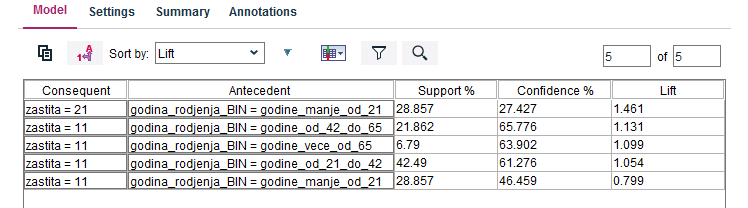
\includegraphics[width=1\textwidth,height=0.15\textheight]{./images/izbor4_apriori.PNG}}
 \caption{Rezultati apriori algoritma primenjenog na kategoriju starosti učesnika i korišćenu zaštitnu opremu. Dolazimo do 
 zaključka da učesnici mladji od 21 godine koriste kacigu kao i da ne nose pojas (doduše oba ova pravila imaju malu pouzdanost). }
\end{figure}

Algoritam carma sa minimalnom podrškom od 20.0\% i minimalnom pouzdanošću 20.0\% nije pronašao zanimljiva pravila (lift mera je veoma
bliska jedinici).

Poslednji pokušaj ticao se traženja povezanosti izmedju ozbiljnosti povrede, izgleda puta na mapi, pozicije nesreće i zaštitne opreme. 
Apriori algoritam je korišćen sa parametrima 5.0\% i 40.0\% za minimalnu podršku i minimalnu pouzdanost, redom. Carma čvor smo koristili
sa podrazumevanim parametrima. 

\begin{figure}[h!]
 \centering
 \makebox[\textwidth][c]{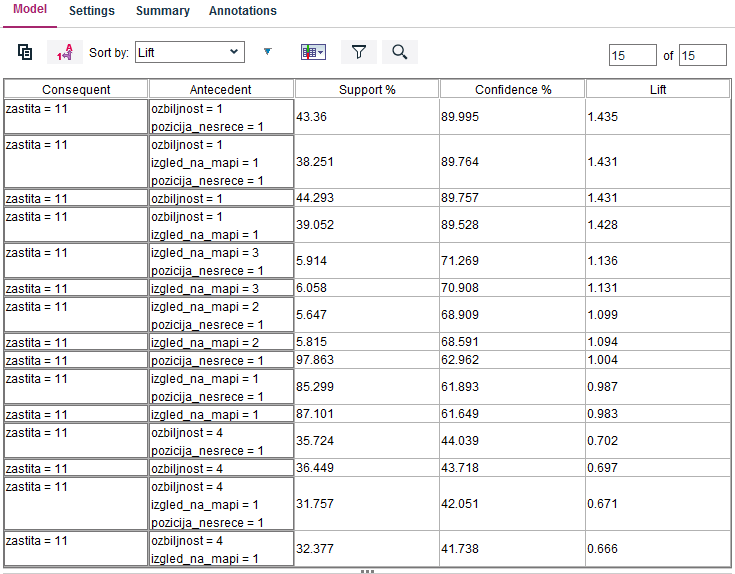
\includegraphics[width=0.8\textwidth,height=0.3\textheight]{./images/izbor5_apriori.PNG}}
 \caption{Rezultati apriori algoritma primenjenog na ozbiljnost povrede, izgled puta na mapi, poziciju nesreće i zaštitnu opremu. 
 Najveći deo pravila kao posledicu ima korišćenje zaštitnog pojasa što je i očekivano s obzirom na broj slogova u kome se pojas 
 javlja, ali smatramo da ovo pravilo ne pruža nikakav značajan zaključak.}
\end{figure}

\begin{figure}[h!]
 \centering
 \makebox[\textwidth][c]{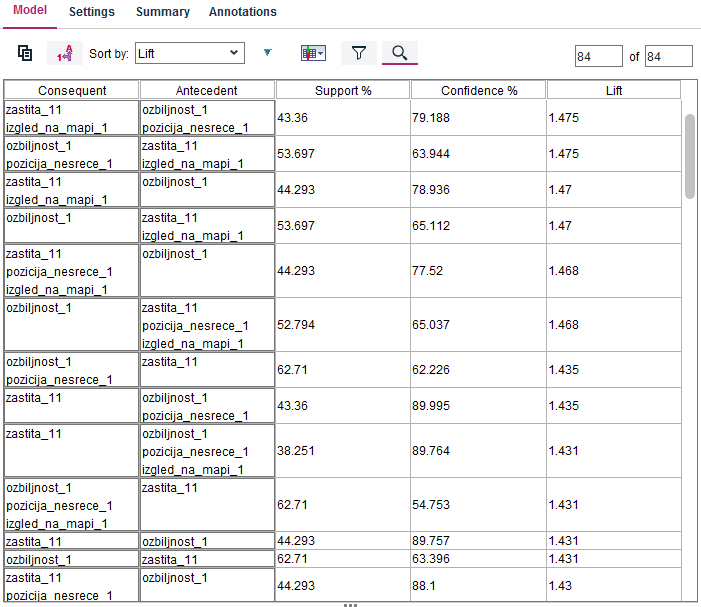
\includegraphics[width=0.8\textwidth,height=0.3\textheight]{./images/izbor5_carma.PNG}}
 \caption{Rezultati carma algoritma primenjenog na ozbiljnost povrede, izgled puta na mapi, poziciju nesreće i zaštitnu opremu. 
 Dobijena pravila imaju dobru lift meru i logična su. Na primer, korišćenje pojasa na pravom putu povezana je sa odsustvom povreda.  }
\end{figure}

\clearpage

\section{Zaključak}

Pravila pridruživanja predstavljaju moćan alat za uočavanje nekih krajnje 
neočekivanih zavisnosti medju podacima. Medjutim, iako su algoritmi za 
nalaženje pravila jednostavni za implementaciju, rezultati dosta zavise i od samih 
podataka. Naime, u poslednje vreme se javljaju radovi koji predlažu naprednije 
tehnike pretprocesiranja kao preduslov za izvlačenje boljih pravila.
U našem slučaju, skup podataka je bio dosta neuravnotežen i smatramo to jednim od 
važnijih faktora za donekle neuspelo pronalaženje interesantnijih pravila.

\end{document}
